\documentclass[11pt, a4paper, twoside]{article}   	% use "amsart" instead of "article" for AMSLaTeX format

\usepackage{geometry}                		% See geometry.pdf to learn the layout options. There are lots.
\usepackage{pdfpages}
\usepackage{caption}
\usepackage{minted}
\usepackage[german]{babel}			% this end the next are needed for german umlaute
\usepackage[utf8]{inputenc}
\usepackage{color}
\usepackage{graphicx}
\usepackage{titlesec}
\usepackage{fancyhdr}
\usepackage{lastpage}
\usepackage{hyperref}
\usepackage[autostyle=false, style=english]{csquotes}
\usepackage{mathtools}
\usepackage{tabularx}
% http://www.artofproblemsolving.com/wiki/index.php/LaTeX:Symbols#Operators
% =============================================
% Layout & Colors
% =============================================
\geometry{
   a4paper,
   total={210mm,297mm},
   left=20mm,
   right=20mm,
   top=20mm,
   bottom=30mm
 }	

\definecolor{myred}{rgb}{0.8,0,0}
\definecolor{mygreen}{rgb}{0,0.6,0}
\definecolor{mygray}{rgb}{0.5,0.5,0.5}
\definecolor{mymauve}{rgb}{0.58,0,0.82}

\setcounter{secnumdepth}{4}


% the default java directory structure and the main packages
\newcommand{\imageDir}{images}
% =============================================
% Code Settings
% =============================================

\newcommand{\xvdash}[1]{%
  \vdash^{\mkern-10mu\scriptscriptstyle\rule[-.9ex]{0pt}{0pt}#1}%
}

% =============================================
% Page Style, Footers & Headers, Title
% =============================================
\title{CLC3 - Cloud Computing}
\author{Marko Gattringer, Christoph Ruhsam}

\lhead{CLC3}
\chead{Cloud Computing}
\rhead{Gattringer, Ruhsam}

\lfoot{}
\cfoot{}
\rfoot{ \thepage / \pageref{LastPage} }
\renewcommand{\footrulewidth}{0.4pt}


\pagestyle{fancy}
\begin{document}
\setlength{\headheight}{15mm}

\section{Dokumentation - CLC3 - Projekt}
Marko Gattringer, Christoph Ruhsam

\subsection{Kurzbeschreibung}
Im Zuge meiner Masterarbeit (Marko Gattringer) wird unter anderem ein Algorithmus entwickelt, welcher einen gezeigten Workflow automatisch aus einem Screencastvideo extrahieren kann. Da dieser Algorithmus sehr rechenintensiv ist (Neuronales Netz mit Tensorflow-GPU) und das Setup dazu nicht trivial ist (Linux, CUDA, Tensorflow-GPU, Python, …), soll dieser als Service angeboten werden. Dazu soll das Service als Microservice angeboten werden und in Openshift (\href{https://www.openshift.com/}{https://www.openshift.com/}) gehostet werden. Weiters dient ein kleine Webapp als Frontend (Login, Verwalten seiner Videos, …). An diesem Beispiel soll gezeigt werden, wie so eine Applikation in Openshift betrieben werden kann. Dabei werden auch Konzepte wie zBsp.: „Infrastructure-as-Code“ oder „Continuous deployment“ umgesetzt.

\section{Ziel / erwartetes Ergebnis}
Microservice-Architektur, welche Lokal (zu Test- und Entwicklungszwecken) als auch in Openshift lauffähig ist.
Angular 8 Frontend, das auch in OpenShift läuft.
Es soll einfach möglich sein, einen Serviceaufruf (auch über mehrere Services hinweg) zu tracen (Jaeger).
Die Build-, Test- und Deploymentvorgänge werden mithilfe von Openshift-Pipelines und Jenkins automatisiert.

\section{Projektstruktur}
\begin{enumerate}
	\item SCAAnalyzerService: Das SCAAnalyzerService ist ein PythonService zum Analysieren von ScreenCasts.
	
	\item SCAPersistService: Das SCAPersistService ist mit Quarkus implementiert. Quarkus ist der Nachfolger von Thorntail, was eine abgespeckte Version des Wildfly war. Quarkus ist eine full-stack, kubernetes-native Java framework und ist darauf optimiert darauf, dass Quarkus-Anwendungen in Kubernetes laufen.
	Es ist eine effektive Plattform für serverless, cloud und Kubernetes Umgebungen.
	Das SCAPersistService bietet dabei die Möglichkeit bereits analysierte Videos in einer MongoDB zu speichern und wieder abzurufen.	
	
	\item SCAAngularFrontend: Das Frontend ist mit Angular 8 implementiert und bietet eine graphische Oberfläche zur Interaktion mit den beiden Service. Grundsätzlich kann sich im Frontend ein User über sein Google-Konto anmelden und dort entweder seine Google-Konto Infos abrufen, ein Video hochladen und dies analysieren oder ein analysiertes Video speichern und in einem Archiv aufrufen.
	
\end{enumerate}

\section{Architektur}
In OpenShift sieht die Architektur wie folgt aus:
\begin{figure}[H]
		\centering
		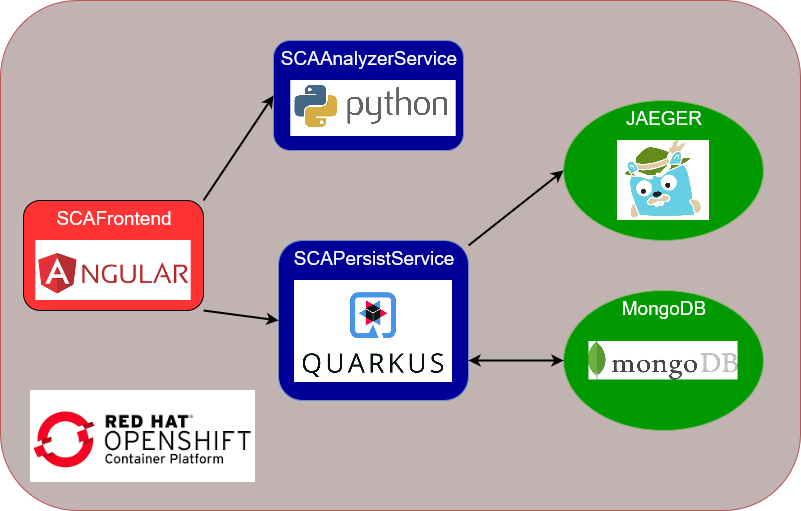
\includegraphics[scale=0.55]{\imageDir/architecture_withOpenshift.png}
		\caption[Architektur OpenShift]
		
\end{figure}

\section{Verwendete Technologien/Bibliotheken}
\begin{itemize}
	\item \href{https://microprofile.io/}{https://microprofile.io/}: Eine Initiative um Java EE für Microsservice-Architekturen zu optimieren. Unterschiedliche Metriken, wie Health, Config, ...
	\item \href{https://www.jaegertracing.io/}{https://www.jaegertracing.io/}: Ein Framework zum Monitoren von Microservices.
	\item \href{https://www.openshift.com/}{https://www.openshift.com/}: Ist eine Container-Plattform von Redhat, welche auf Docker und Kubernetes aufbaut.
	\item \href{https://jenkins.io/}{https://jenkins.io/}: Automation Server für automatisierte Build-, Test- und Deploymentvorgänge.
\end{itemize}

\section{Setup}
\begin{enumerate}
	\item TODO Codeready Container
	\item In gewünschtes Verzeichnis entpacken und PATH Variable um dieses Verzeichnis erweitern
	\item Docker starten (muss laufen damit Openshift Cluster gestartet werden kann, basiert auf Docker-Images)
	\item \textbf{oc cluster up}: startet einen neuen Cluster
	\item \textbf{oc login}: am lokalen Cluster anmelden (fabric8 deployed in den Cluster an dem man aktuell eingeloggt ist) -> USER/PASSWORT kann beliebig gewählt werden
	\item \textbf{oc new-project [PROJEKTNAME]}: Legt ein neues Projekt an
	\item \textbf{oc process -f https://raw.githubusercontent.com/jaegertracing/jaeger-openshift/master/all-in-one/jaeger-all-in-one-template.yml | oc create -f -}: Deployt ein vorgefertigtes Jaeger Template
	\item \textbf{oc process -f https://raw.githubusercontent.com/sabre1041/openshift-api-swagger/master/openshift-api-swagger-template.yml | oc apply -f-}: Deployt ein vorgefertigtes SwaggerUI Template
\end{enumerate}

\section{OpenShift}
OpenShift ist eine OpenSource Container Application Platform und setzt auf Kubernetes auf.
Nach dem Befehl \textbf{oc cluster up} kann unter \textit{localhost:8443} die grafische Oberfläche aufgerufen werden.
Sind bereits Services in OpenShift deployt, sieht dies wie folgt aus:
TODO image from OpenShift

Ein Service kann auf hinauf-/heruntergescaled werden. Dadurch können mehrere Pods gestartet werden. Das Load-Balancing wird von OpenShift übernommen.
TODO image from OpenShift Projekt

\begin{figure}[H]
	\centering
	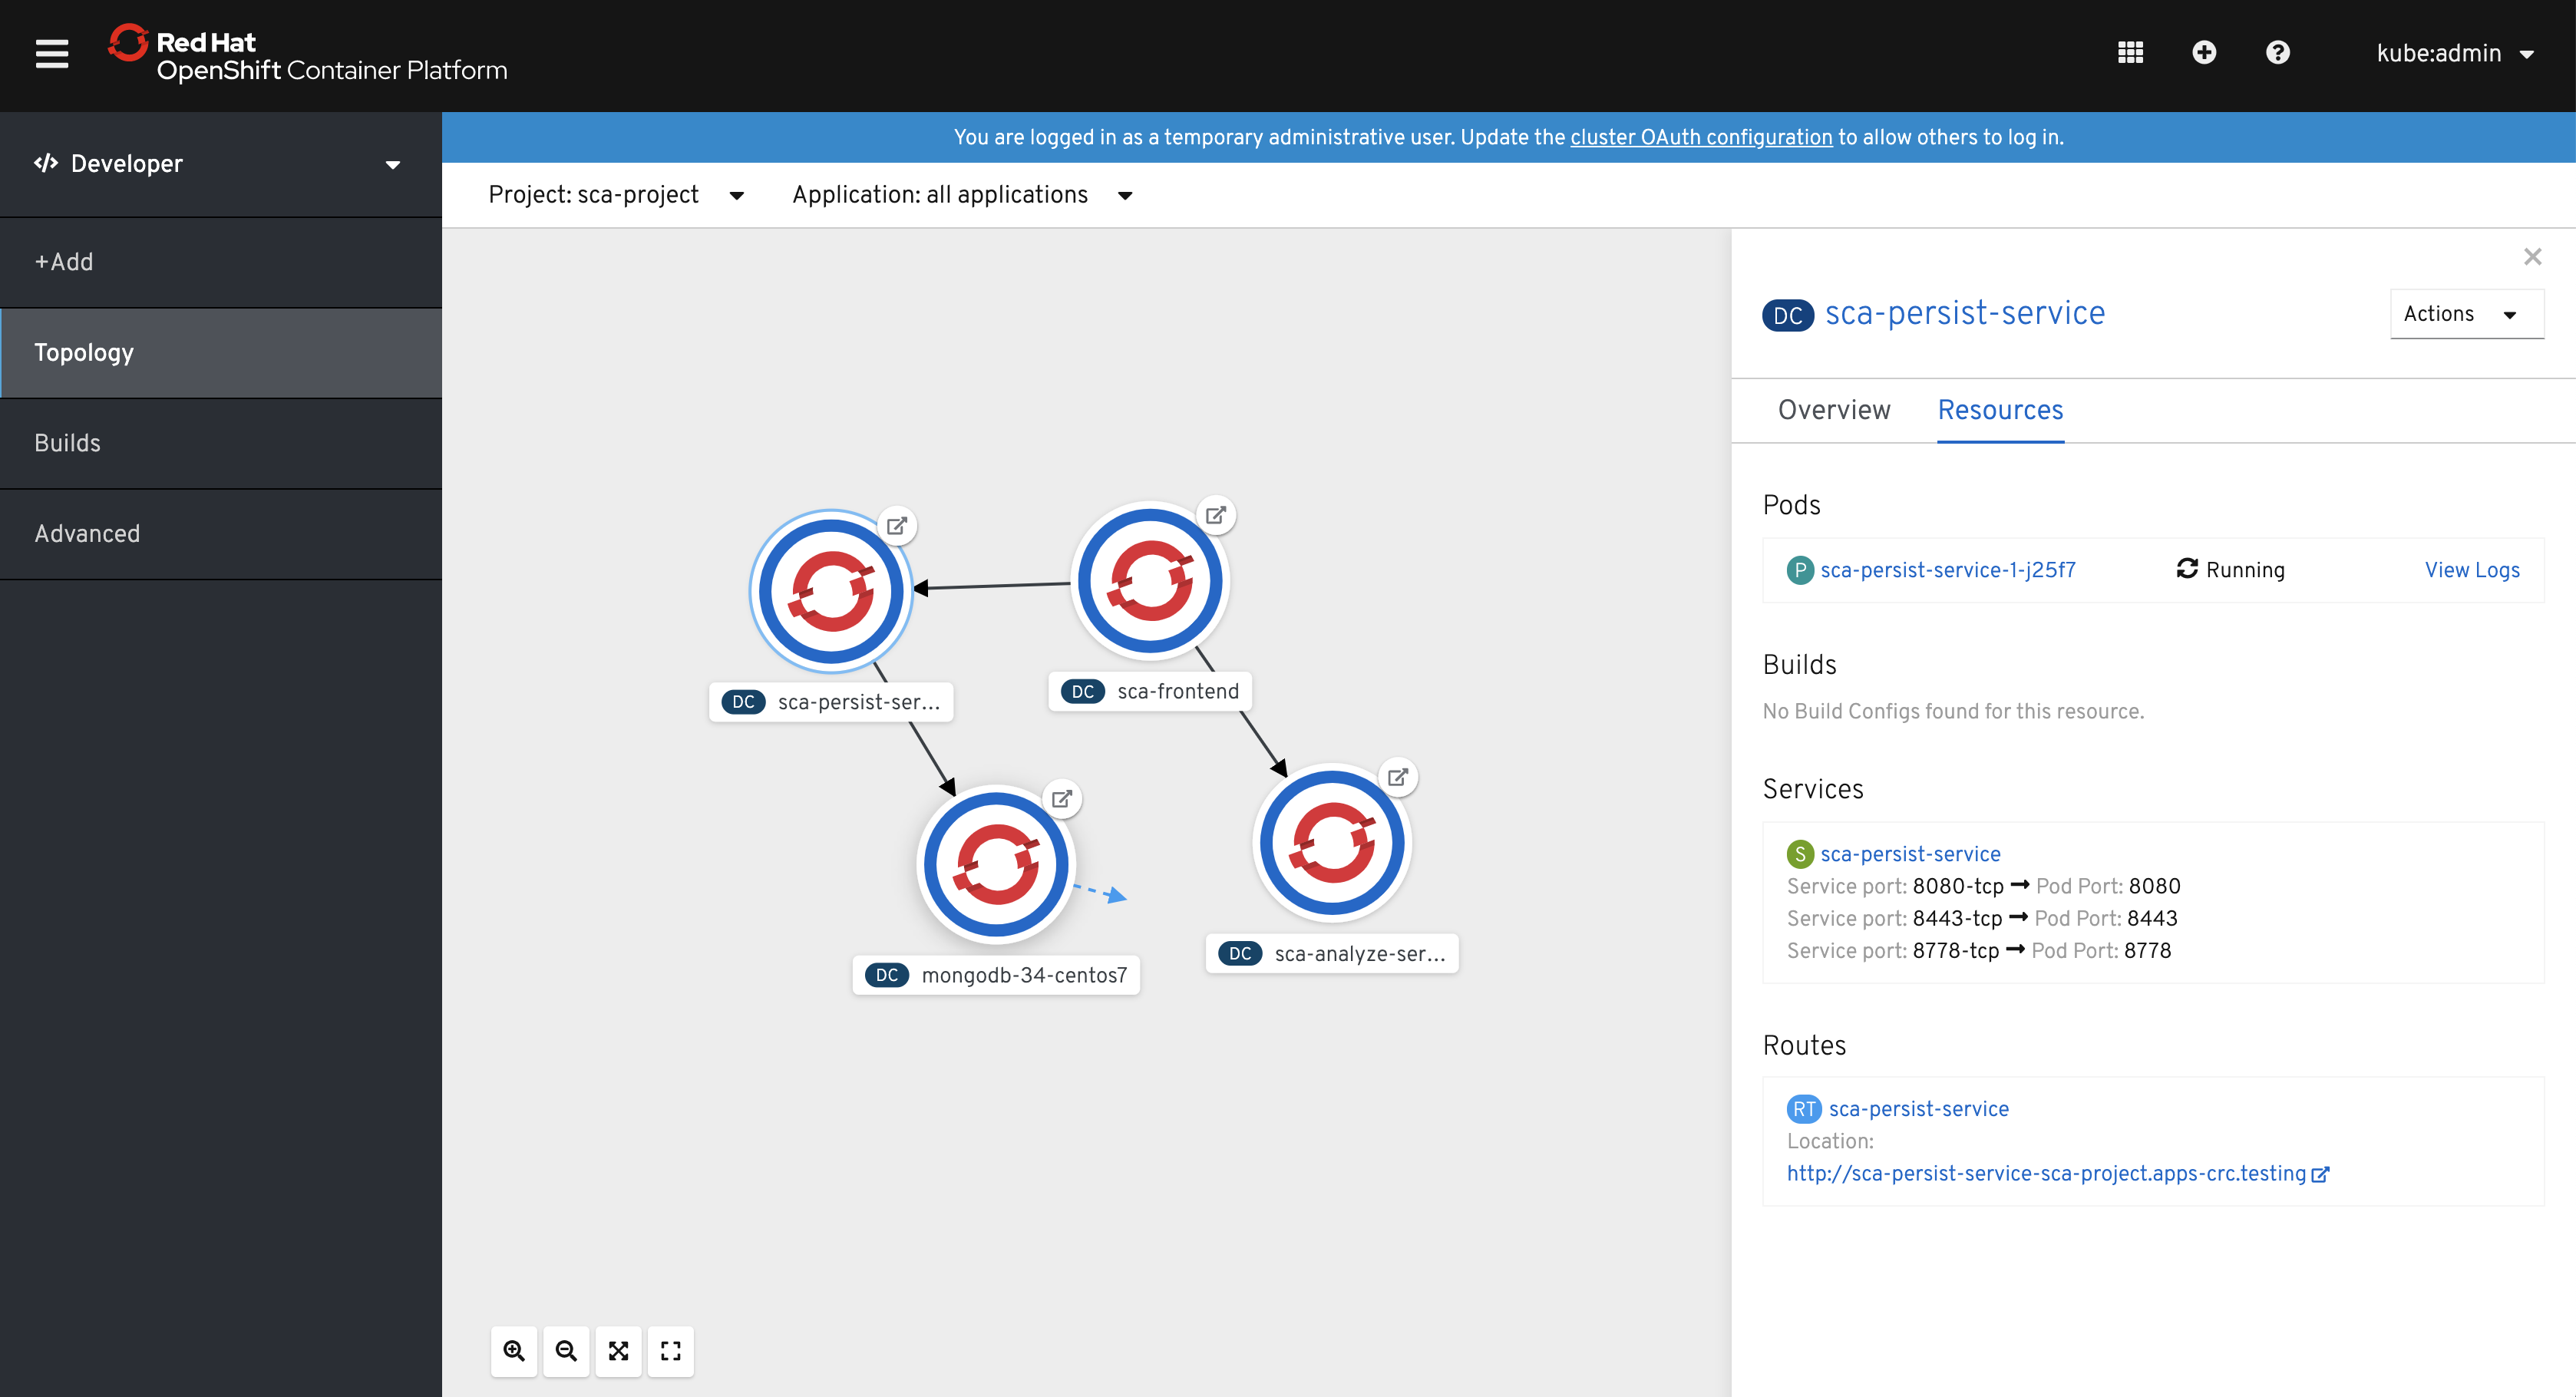
\includegraphics[scale=0.25]{\imageDir/openshift_overview.png}
	\caption[OpenShift]
	
\end{figure}

\section{OpenTracing mit Jaeger}
Jaeger ist ein Tracing System, das OpenSource zur Verfügung steht. Es wird für Monitoring und Troubleshooting bei Microservice-Architekturen verwendet.
Um Jaeger mit Thorntail und JavaEE verwenden zu können, werden folgende Teile benötigt:
\begin{itemize}
	\item io.quarkus.quarkus-smallrye-opentracing  Dependency
	\item Im application.properties folgende Konfigurationsparameter:
	\begin{itemize}
		\item service-name: Service Name der mit den Spans assoziiert wird
		\item agent-host: Host unter dem der jaeger-agent erreichbar ist
		\begin{itemize}
			\item Dieser ist für die lokale Entwicklung localhost
			\item Und in OpenShift \textbf{NICHT} die Route von Jaeger, sondern der Container Name von Jaeger. In unserem Fall jaeger-agent.
		\end{itemize}
		\item agent-port: Port unter dem der jaeger-agent erreichbar ist.
		\item reporter-flush-interval: Definiert, wie oft Jaeger die Spans flusht
		\item sampler-type: Definiert den Typ des Samplers, z.B.: probabilistic oder const
		\item sampler-parameter: Configurations-Wert für den Sampler, z.B.: probabilistic = 0.001
	\end{itemize}
\end{itemize} 

Ist Jaeger und ein Service deployed und eine getracte REST-Resource dieses Service wird aufgerufen, wird der Span an Jaeger gesendet. Mittels der JaegerUI, deren URL in OpenShift zu sehen ist, können die Traces angesehen werden.

\section{MongoDB}
Deployen und Starten der MongoDB in OpenShift: \newline
\textit{oc new-app -e MONGODB\_USER=test -e MONGODB\_PASSWORD=test -e MONGODB\_DATABASE=sca -e MONGODB\_ADMIN\_PASSWORD=test openshift/mongodb-24-centos7} \newline
Exposen der Route: \newline
\textit{oc expose svc/mongodb-24-centos7}

\section{Fragestellungen}
\subsection{Automated Infrastructue Provisioning/(Infrastructure-as-Code). Wie wurde im vorliegenden Projekt Automated Infrastructure Provisioning berücksichtigt?}
Beim Deployen der Services erzeugt OpenShift ein \textbf{deployment.yaml} mit Standardwerten. Dieses kann je nach Bedarf modifiziert werden. Werden nun System mit diesem deployment.yaml erzeugt, bleiben diese konsistent. Solange Änderungen auch nur in diesem Konfigurations-File durchgeführt werden, bleibt das System auch konsistent und kann jederzeit reproduziert werden.
Dadurch werden die 4 folgenden Grundsätze von Infrastructure as Code in unserem Projekt umgesetzt.

\begin{itemize}
	\item Systeme sind reproduzierbar
	\item Systeme sind wegwerfbar
	\item Systeme sind konsistent
	\item Aktionen sind wiederholbar
\end{itemize}


\subsection{Skalierbarkeit. Wie wurde im vorliegenden Projekt Skalierbarkeit berücksichtigt?}
\begin{figure}[H]
	\centering
	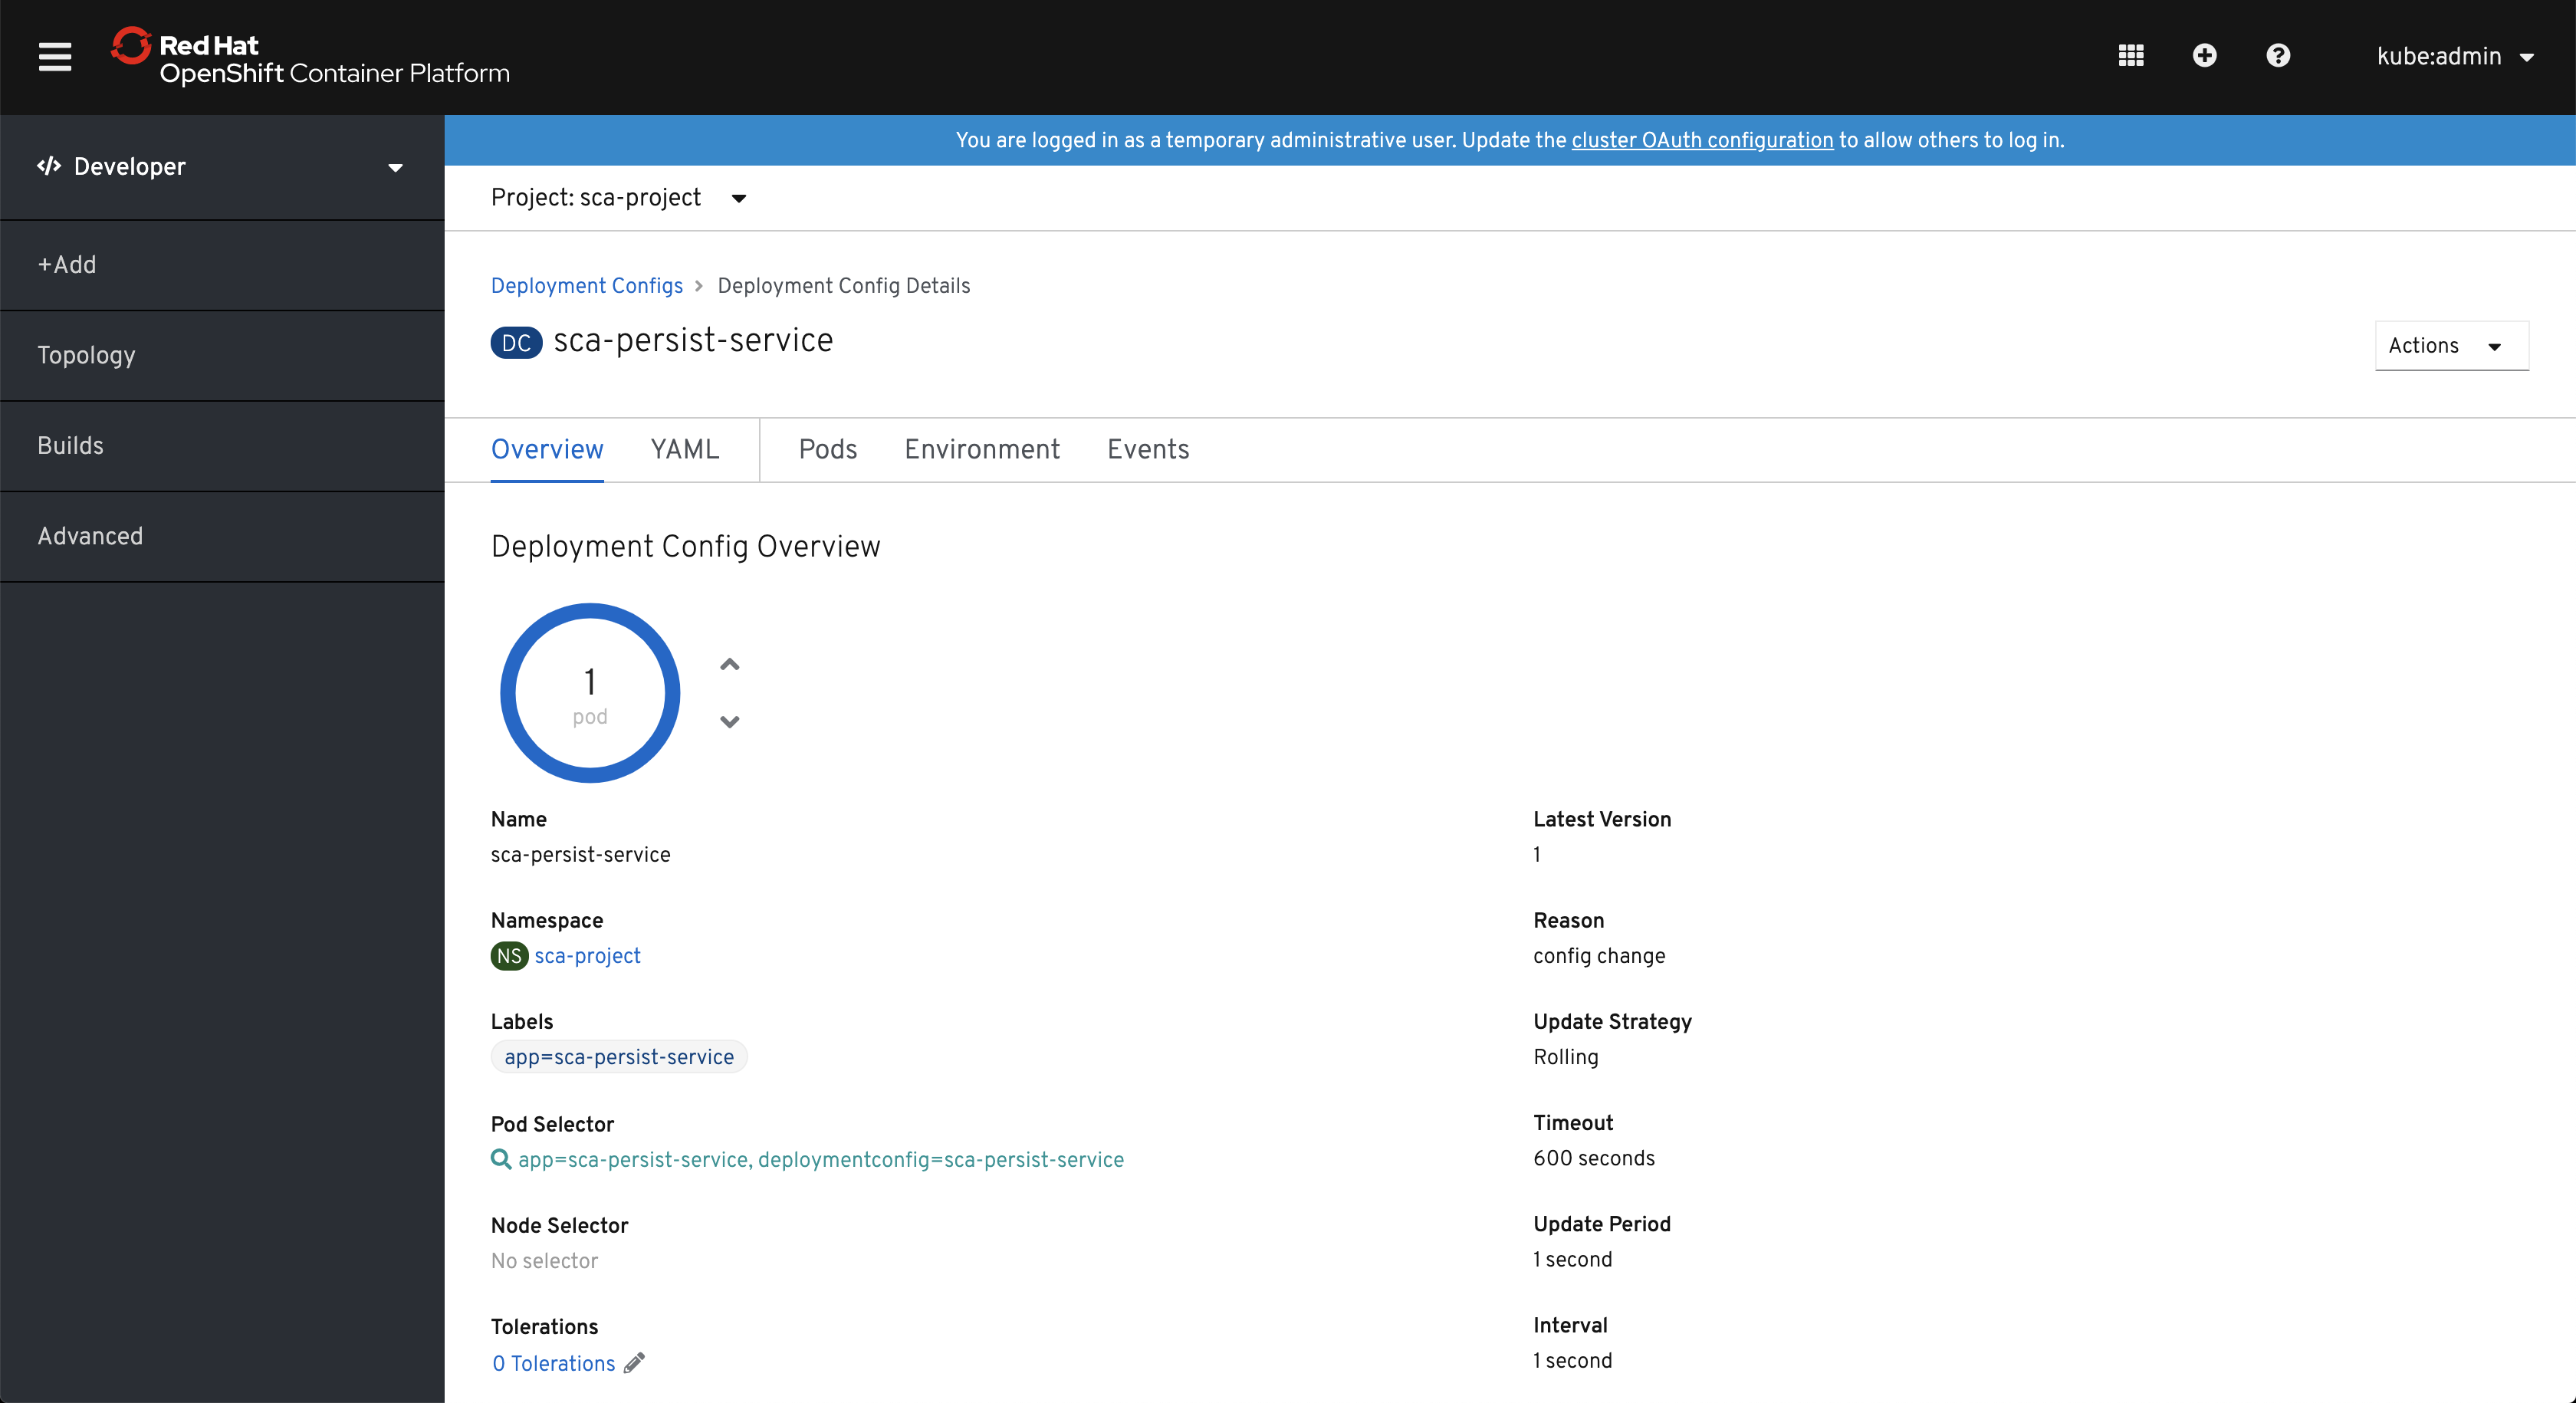
\includegraphics[scale=0.27]{\imageDir/service_scale_up.png}
	\caption[Scale Up- Funktion]
\end{figure}


\subsection{Ausfallssicherheit.  Wie wurde im vorliegenden Projekt Ausfallssicherheit berücksichtigt?}


\subsection{NoSql. Welchen Beitrag leistet NoSql in der vorliegenden Problemstellung?}


\subsection{Replikation. Wo nutzen Sie im gegenständlichen Projekt Daten-Replikation?}

\subsection{Kosten. Welche Kosten verursacht Ihre Lösung? Welchen monetären Vorteil hat diese Lösung gegenüber einer Nicht-Cloud-Lösung?}
\end{document}